% ITY – projekt 5
% Ondřej Ondryáš (xondry02), FIT VUT
% Datum: 3. 5. 2020
% Využil jsem FIT šablonu pro beamer dostupnou na https://www.fit.vut.cz/study/theses/master-theses/.cs.
% Tato šablona bohužel způsobuje nějaké overfull hbox chyby (myslím, že je to způsobeno vkládáním loga FIT)
% a jednu underfull vbox chybu na titulní stránce, nemyslím si ale, že to je podstatné.

\documentclass[10pt,xcolor=pdflatex,hyperref={unicode,hidelinks}]{beamer}

\usepackage{newcent}
\usepackage[utf8]{inputenc}
\usepackage[T1]{fontenc}
\usepackage[czech]{babel}
\usepackage{amsmath,amsfonts,amssymb}
\usepackage{fancyvrb}
\usepackage{url}
\usepackage{algorithmicx}
\usepackage[noend]{algpseudocode}
\usepackage{mathtools}
\usepackage{ragged2e}
\usetheme{FIT}

\usepackage{tikz}

\usetikzlibrary{graphs,graphs.standard,arrows.meta,automata,positioning,quotes}

\deftranslation[to=czech]{Definition}{Definice}

\title[Grafové algoritmy]{Vyhledávání nejkratší cesty v~grafu}

\author[]{Ondřej Ondryáš}

\institute[]{Fakulta informačních technologií VUT v~Brně\\
Bo\v{z}et\v{e}chova 1/2, 612 66 Brno - Kr\'alovo Pole\\
xondry02@stud.fit.vutbr.cz}

\date{\today}

\begin{document}

\frame[plain]{\titlepage}
\begin{frame}\frametitle{Graf -- opakování}
    \begin{itemize}
        \item<1-> \emph{Graf} se dá chápat jako:
        \begin{itemize}
            \item<2-> nakreslená relace
            \item<3-> dvojice množiny vrcholů a množiny hran
        \end{itemize}
        \item<4-> Jak by se daly zapsat tyto grafy?
    \end{itemize}
    
    \begin{columns}<4->
    \column{0.5\textwidth}
    \begin{figure}
        \centering
        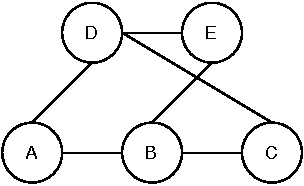
\includegraphics[width=3cm]{img/graf_neori.pdf}
        \\\emph{Neorientovaný} graf $N$
    \end{figure}
    \column{0.5\textwidth}
    \begin{figure}
        \centering
        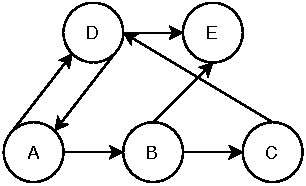
\includegraphics[width=3cm]{img/graf_ori.pdf}
        \\\emph{Orientovaný} graf $O$
    \end{figure}
    \end{columns}
    
    \begin{itemize}
        \item<5-> $N$ jako množina dvouprvkových množin, které reprezentují jednotlivé dvojice vrcholů:
        \begin{itemize}
            \item<6-> $N = \{\{A, D\}, \{A, B\}, \{D, E\}, \{D, C\}, \{E, B\}, \{B, C\}\}$
        \end{itemize}
        \item<7-> $O$ jako relace:
        \begin{itemize}
            \item<8-> $O = \{[A, D], [D, A], [A, B], [D, E], [C, D], [B, E], [B, C]\}$
        \end{itemize}
    \end{itemize}
\end{frame}

\begin{frame}\frametitle{Graf -- opakování}
    \begin{definition}
        \emph{Neorientovaný graf} je \emph{uspořádaná dvojice} $G = (V, E)$, kde $V$ je množina \emph{vrcholů} a $E$ je množina dvouprvkových podmnožin množiny vrcholů, tzv. (neorientovaných) \emph{hran}.
    \end{definition}
    
    \begin{itemize}
        \item<2-> Vrcholy spojené hranou jsou \emph{sousední} a hrana $\{u, v\}$ \emph{vychází} z~vrcholů $u$ a $v$.
    Na množinu vrcholů grafu $G$ ukazujeme pomocí $V(G)$, na množinu hran pomocí $E(G)$.
        \item<2-> Neorientovaný graf obvykle označujeme pouze jako \emph{graf}. Orientovaný graf se někdy označuje jako \emph{digraf}.
    \end{itemize}
\end{frame}

\begin{frame}\frametitle{Graf -- opakování}
    \begin{definition}
        \emph{Cesta} délky $n \geq 0$ je posloupnost $P = (v_0, e_1, v_1,\ldots, e_n, v_n)$, pro kterou platí $e_i = \{ v_{i-1}, v_i \} \wedge v_i\ne v_j \text{ pro } i \ne j$.
    \end{definition}
    
    \begin{itemize}
        \item<2-> Cesta je tedy posloupnost $n + 1$ vrcholů za sebou spojených $n$ hranami.
    \end{itemize}
\end{frame}

\begin{frame}\frametitle{Vážený graf}
    \begin{itemize}
        \item<1-> {Mějme funkci $len$, která jednotlivým hranám $e \in E(G)$ grafu $G$ přiřazuje reálná čísla -- \emph{ohodnocení}:
        \[
            len: E(G) \rightarrow \mathbb{R}
        \]
        
        Dvojici $(G, len)$ sestávající z~grafu a ohodnocovací funkce můžeme označit jako \emph{vážený graf}.}
        \item<2-> {\emph{Vážená délka cesty $P$} ve váženém grafu $(G, len)$ je součet vah jejích hran: 
        \[
            d^{len}_G(P) = \sum_{e \in E(P)} len(e)
        \]}
        \item<2-> {\emph{Vážená vzdálenost} mezi vrcholy $u$ a $v$ je vážená délka \textbf{nejkratší cesty} mezi nimi:
        \[
            d^{len}_G(u, v) = \min\{d^{len}_G(P) \text{, kde } P \text{ je cestou z~} u~\text{ do } v\}
        \]}
    \end{itemize}
\end{frame}

\begin{frame}[t]\frametitle{Problém}
    \begin{columns}[T,onlytextwidth]
    \column{\dimexpr\linewidth-29mm-5mm}
    \begin{itemize}
        \item<1-> Zoufalý student hledá nejkratší cestu z~fakulty \emph{M} na fakultu \emph{V}.
        \item<2-> Město je nechvalně známé nevyhovujícím stavem svých cest.
        \item<3-> Navigační aplikace zná polohu všech křižovatek\ldots
        \item<4-> \ldots\ a úseky mezi nimi ohodnotila podle vzdálenosti a stavu sjízdnosti.
        \item<5-> \emph{Jakou cestu má studentovi aplikace doporučit?}
        \item<6-> Potřebujeme algoritmus, který najde cestu $P$ mezi dvěma vrcholy grafu s~nejkratší váženou délkou.
    \end{itemize}
    
    \column{29mm}
    \centering
    \only<1>{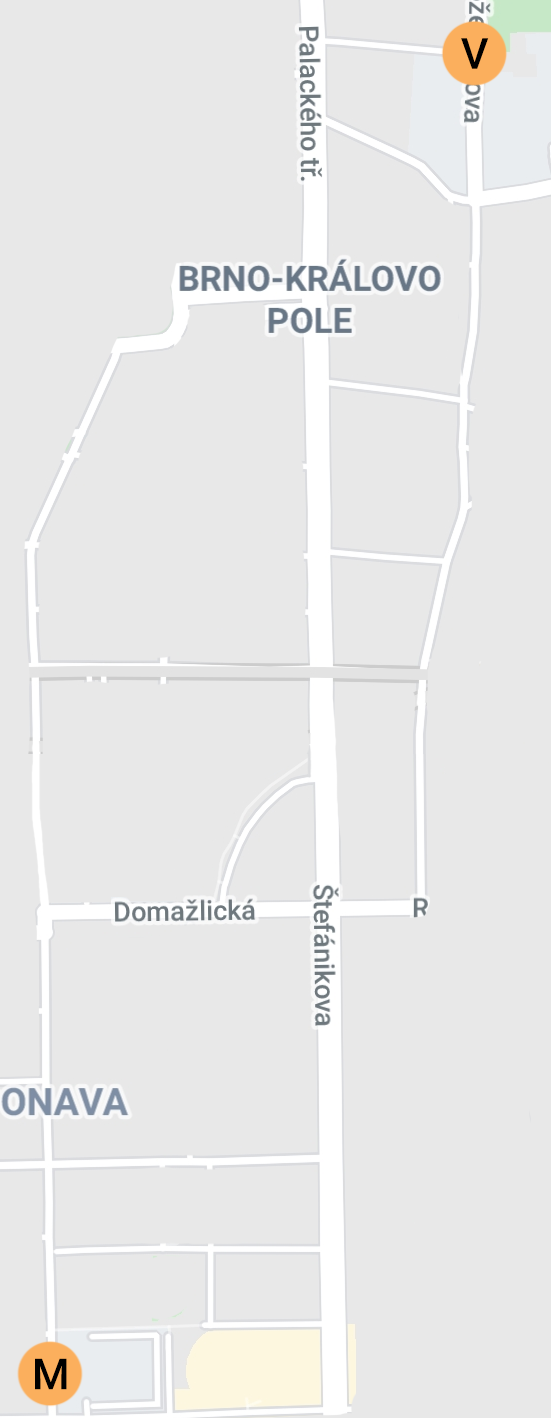
\includegraphics[width=29mm]{img/map/stud_empty_map.png}}
    \only<2>{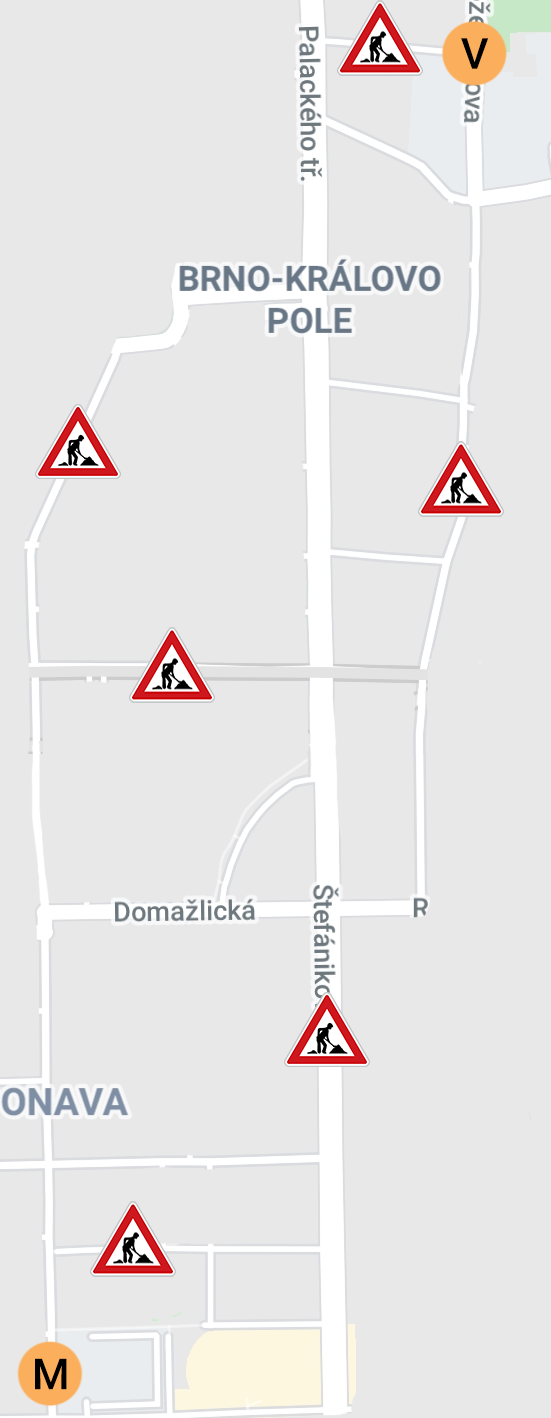
\includegraphics[width=29mm]{img/map/stud_dangers_map.png}}
    \only<3>{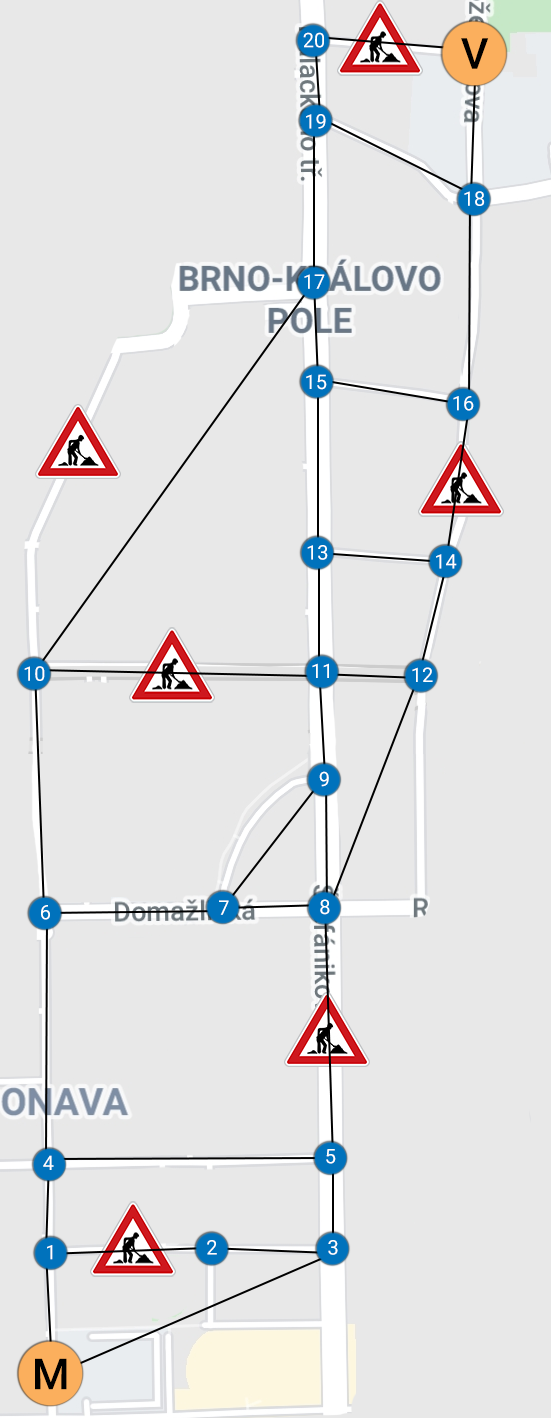
\includegraphics[width=29mm]{img/map/stud_graph.png}}
    \only<4->{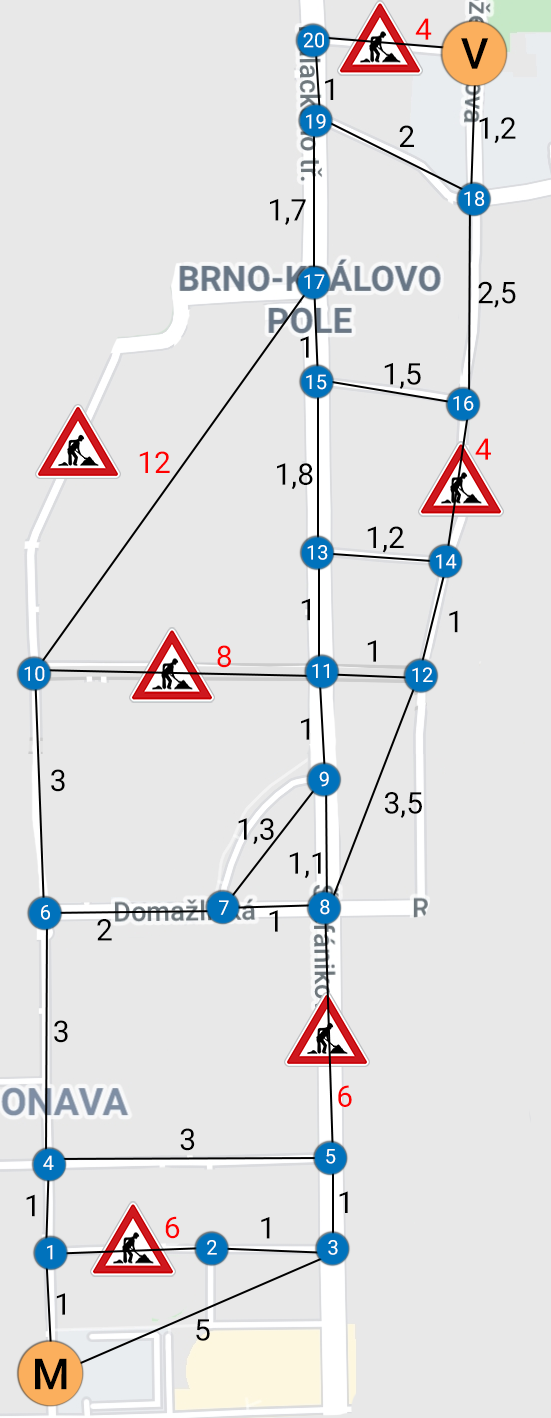
\includegraphics[width=29mm]{img/map/stud_graph_vals.png}}
    \end{columns}
\end{frame}

\begin{frame}\frametitle{Problém}
    \centering
    \begin{tikzpicture}
\tikzset{st/.style={draw=orange, minimum size=0.8cm}}
\tikzset{pth/.style={draw=red, minimum size=0.8cm}}

\begin{scope}[scale=0.7,every node/.style={circle,thick,draw}]
\node [st] (M) at (7.3,10.0) {M};
\node [st] (V) at (1.4,0.2) {V};
\node (1) at (4.3,9.4) {1};
\node (2) at (6.6,8.1) {2};
\node (3) at (9.4,8.2) {3};
\node (4) at (4.6,7.2) {4};
\node (5) at (7.6,6.6) {5};
\node (6) at (2.6,6.0) {6};
\node (7) at (6.0,5.6) {7};
\node (8) at (10.0,5.9) {8};
\node (9) at (8.4,4.5) {9};
\node (10) at (4.2,4.3) {10};
\node (11) at (6.5,3.6) {11};
\node (12) at (10.0,3.3) {12};
\node (13) at (7.9,2.1) {13};
\node (14) at (9.9,0.8) {14};
\node (15) at (4.9,2.2) {15};
\node (16) at (6.9,0.3) {16};
\node (17) at (1.8,3.9) {17};
\node (18) at (4.2,0.0) {18};
\node (19) at (2.8,2.0) {19};
\node (20) at (0.0,2.4) {20};
\end{scope}
\begin{scope}[>={Stealth[black]},scale=0.7,every node/.style={fill=white,font=\footnotesize},every edge/.style={draw=black,very thick}]
\path (M) edge node {$1$} (1);
\path (M) edge[red] node {$5$} (3);
\path (1) edge[red] node {$6$} (2);
\path (2) edge node {$1$} (3);
\path (1) edge node {$1$} (4);
\path (4) edge node {$3$} (5);
\path (3) edge node {$1$} (5);
\path (4) edge node {$3$} (6);
\path (5) edge[red] node {$6$} (8);
\path (6) edge node {$2$} (7);
\path (7) edge node {$1$} (8);
\path (7) edge node {$1.3$} (9);
\path (8) edge node {$1.1$} (9);
\path (8) edge node {$3.5$} (12);
\path (11) edge node {$1$} (12);
\path (10) edge[red] node {$8$} (11);
\path (9) edge node {$1$} (11);
\path (11) edge node {$1$} (13);
\path (13) edge node {$1.2$} (14);
\path (12) edge node {$1$} (14);
\path (14) edge[red] node {$4$} (16);
\path (13) edge node {$1.8$} (15);
\path (15) edge node {$1.5$} (16);
\path (15) edge node {$1$} (17);
\path (10) edge[red] node {$12$} (17);
\path (16) edge node {$2.5$} (18);
\path (17) edge node {$1.7$} (19);
\path (18) edge node {$2$} (19);
\path (19) edge node {$1$} (20);
\path (18) edge node {$1.2$} (V);
\path (20) edge[red] node {$4$} (V);
\end{scope}

\end{tikzpicture}
\end{frame}

\begin{frame}\frametitle{Dijkstrův algoritmus}
    \begin{itemize}
        \item<1-> S~jedním z~možných řešení problému nalezení nejkratší cesty přišel v~roce 1956 nizozemský informatik Edsger W.~Dijkstra.
        \item<2-> Jednoduchý princip:
            \begin{enumerate}
                \item<2-> Všem vrcholům je přiřazena vzdálenost od počátečního vrcholu, na začátku počáteční vrchol 0, ostatní „nekonečno“.
                \item<3-> Algoritmus vybere vrchol $v$ s~\textbf{nejnižší aktuálně přiřazenou vzdáleností}.
                \item<4-> Pro všechny sousední vrcholy je určena vzdálenost, kterou by měly, kdyby byl jejich předchůdcem vrchol $v$.
                \item<5-> Pokud je tato vzdálenost nižší než aktuálně přiřazená vzdálenost, vrcholu je tato vzdálenost přiřazena a jako jeho předchůdce je nastaven $v$.
            \end{enumerate}
        \item<6-> Existují různé variace a možnosti implementace.
        \item<7-> S~použitím vhodných datových struktur dosahuje uspokojivé asymptotické časové složitosti $O(|E| + |V| \log|V|)$.
        \item<8-> Použitelný pouze pro \textbf{kladně vážené grafy}.
    \end{itemize}
\end{frame}

\shorthandoff{"}
\tikzset{
    invisible/.style={opacity=0},
    visible on/.style={alt=#1{}{invisible}},
    alt/.code args={<#1>#2#3}{%
      \alt<#1>{\pgfkeysalso{#2}}{\pgfkeysalso{#3}} % \pgfkeysalso doesn't change the path
    },
}
    
\begin{frame}\frametitle{Dijkstrův algoritmus: demonstrace}
    \centering
    \begin{tikzpicture}[
    node distance = 22mm,
    every state/.append style = {inner sep=0pt, fill=gray!10,
                                 minimum size=7mm},
    every edge/.style = {draw, bend angle=15},auto=right]
    
    \tikzset{foundEdge/.style={gray!30, line width=5pt}}
    \tikzset{done/.style={state, fill=green!75}}
    \tikzset{gre/.style={state, fill=gray!50}}
    
    \node (s1) [visible on=<1>,   gre]                       {0};
    \node (s1) [visible on=<2->, done]                       {0};
    
    \node (s2) [visible on=<1>,  state, above right=of s1]   {$\infty$};
    \node (s2) [visible on=<2>,    gre, above right=of s1]   {2?};
    \node (s2) [visible on=<3->,  done, above right=of s1]   {2};
    
    \node (s3) [visible on=<1-2>,state, right=of s2]         {$\infty$};
    \node (s3) [visible on=<3-5>,  gre, right=of s2]         {8?};
    \node (s3) [visible on=<6->,  done, right=of s2]         {8};
    
    \node (s4) [visible on=<1-3>,state, below right=of s3]   {$\infty$};
    \node (s4) [visible on=<4-5>,  gre, below right=of s3]   {12?};
    \node (s4) [visible on=<6>,    gre, below right=of s3]   {10?};
    \node (s4) [visible on=<7>,   done, below right=of s3]   {10};
    
    \node (s5) [visible on=<1-2>,state, below  left=of s4]   {$\infty$};
    \node (s5) [visible on=<3>,    gre, below  left=of s4]   {5?};
    \node (s5) [visible on=<4->,  done, below  left=of s4]   {5};
    
    \node (s6) [visible on=<1>,  state, left=of s5]          {$\infty$};
    \node (s6) [visible on=<2->,   gre, left=of s5]          {8?};
    \node (s6) [visible on=<3>,    gre, left=of s5]          {7?};
    \node (s6) [visible on=<4>,    gre, left=of s5]          {6?};
    \node (s6) [visible on=<5->,  done, left=of s5]          {6};
    
    %
    \draw[foundEdge, visible on=<2->]
            (s1) to                     (s2);
    \draw[foundEdge, visible on=<2>]
            (s1) to                     (s6);
    \draw[foundEdge, visible on=<3>]
            (s2) to                     (s6);
    \draw[foundEdge, visible on=<3->]
            (s2) to                     (s3);
    \draw[foundEdge, visible on=<3->]
            (s2) to                     (s5);
    \draw[foundEdge, visible on=<4->]
            (s5) to                     (s6);
    \draw[foundEdge, visible on=<4-5>]
            (s5) to                     (s4);
    \draw[foundEdge, visible on=<6->]
            (s3) to                     (s4);
    %
    \draw   (s1) edge ["2"]             (s2)
            (s1) edge ["8"]             (s6)
            (s2) edge ["6"]             (s3)
            (s2) edge ["3"]             (s5)
            (s2) edge ["5"]             (s6)
            (s3) edge ["2"]             (s4)
            (s3) edge ["5"]             (s5)
            (s5) edge ["7"]             (s4)
            (s5) edge ["1"]             (s6);
\end{tikzpicture}
\end{frame}
\shorthandon{"}

\algnewcommand\algorithmicforeach{\textbf{for each}}
\algdef{S}[FOR]{ForEach}[1]{\algorithmicforeach\ #1\ \algorithmicdo}

\begin{frame}\frametitle{Dijkstrův algoritmus: pseudokód}
    Vstupem je vážený graf $(G, len)$ a počáteční vrchol $a$. $dist$ a $prev$ jsou struktury, které pro klíč typu \textit{vrchol} drží hodnotu typu \textit{číslo}, resp. \textit{vrchol}.
    \begin{algorithmic}[1]
        \ForEach{$x \in V(G)$}
            \State $dist(x)\gets \infty$
            \State $prev(x)\gets NULL$
        \EndFor
        
        \State $dist(a)\gets 0$
        \State $Q = \{a\}$
        
        \While{$Q\not=\emptyset$}
            \State $u\gets$ vrchol z~$Q$ s~minimální $dist(u)$
            \State \textbf{remove} $u$ \textbf{from} $Q$\label{dijkstra_stop}
            \ForEach{hrana $\{u, v\} \in E(G)$}
                \State $possible\_dist \gets dist(u) + len(\{u, v\})$ 
                \If{$possible\_dist < dist(v)$}
                    \State $dist(v) \gets possible\_dist$
                    \State $prev(v) \gets u$
                    \State $Q \gets v$
                \EndIf
            \EndFor
        \EndWhile
    \end{algorithmic}
\end{frame}

\begin{frame}\frametitle{Dijkstrův algoritmus: rozbor}
    \only<1>{
    Na začátku se pro všechny vrcholy grafu nastaví příslušný záznam v~$dist$ na $\infty$ (neznámá vzdálenost) a v~$prev$ na $NULL$ (neznámý předchůdce).
    
    \begin{algorithmic}[1]
        \ForEach{$x \in V(G)$}
            \State $dist(x)\gets \infty$
            \State $prev(x)\gets NULL$
        \EndFor
        \algstore{rozbor}
    \end{algorithmic}
    
    Pro počáteční vrchol $a$ nastavíme nulovou vzdálenost a~vytvoříme množinu $Q$, která drží \textit{„zlepšené“} vrcholy -- vrcholy, ke kterým už byla přiřazena vzdálenost, ale nebylo prohledáno jeho okolí. 
    
    \begin{algorithmic}[1]
        \algrestore{rozbor}
        \State $dist(a)\gets 0$
        \State $Q = \{a\}$
        \algstore{rozbor}
    \end{algorithmic}  
    }
    
    \only<2>{
    Dokud není $Q$ prázdná, vybíráme (a odstraňujeme) z~ní vrchol $u$ s~aktuálně nejnižší přiřazenou vzdáleností.
    
    \begin{algorithmic}[1]
        \algrestore{rozbor}
        \While{$Q\not=\emptyset$}
            \State $u\gets$ vrchol z~$Q$ s~minimální $dist(u)$
            \State \textbf{remove} $u$ \textbf{from} $Q$
        \algstore{rozbor}
    \end{algorithmic}
    }
    
    \only<3>{
    Procházíme sousedy $v$ vrcholu $u$. Pro každý z~nich zjistíme, jaká by byla jeho vzdálenost, pokud bychom se k~němu dostali „přes~$u$“ -- součet vzdálenosti $u$ a váhy hrany spojující $u$ s~$v$. Pokud je tato vzdálenost menší než aktuálně nastavená vzdálenost $v$, nastavíme ji a jako předchůdce nastavíme $u$. Přidáme $v$ do $Q$ (pokud tam už není), vrchol $v$ se tak stane kandidátem pro výchozí vrchol prohledávání v~další iteraci. Je možné dokázat, že pokud se tak stane, k~vrcholu $v$ už je nalezena nejkratší cesta.
    \begin{algorithmic}[1]
        \algrestore{rozbor}
            \ForEach{hrana $\{u, v\} \in E(G)$}
                \State $possible\_dist \gets dist(u) + len(\{u, v\})$ 
                \If{$possible\_dist < dist(v)$}
                    \State $dist(v) \gets possible\_dist$
                    \State $prev(v) \gets u$
                    \State $Q \gets v$
                \EndIf
            \EndFor
        \EndWhile
    \end{algorithmic}
    }
\end{frame}

\begin{frame}\frametitle{Dijkstrův algoritmus: poznámky}
    \begin{itemize}
        \item<1-> Pokud hledáme pouze cestu mezi dvěma body, je možné ukončit prohledávání za řádkem \ref{dijkstra_stop}, pokud se vyjmutý vrchol $u$ rovná cílovému vrcholu.
        \item<2-> Uvedený algoritmus ukládá do $Q$ vrcholy, až když na ně při prohledávání poprvé narazí. Asymptotickou složitostí ekvivalentní možností je uložit do $Q$ na začátku všechny vrcholy, v~takovém případě je ale fronta větší a v~praxi je tak její procházení časově náročnější.
        \item<3-> Implementace operace vyhledání vrcholu s~minimální $dist(u)$ představuje možnost optimalizace algoritmu. Při použití lineárního prohledávání a implementaci $Q$ jako fronty je asymptotická složitost $O(|E| + |V|^2)$.
    \end{itemize}
\end{frame}

\begin{frame}\frametitle{A co zoufalý student?}
    \centering
    \only<1>{
    \resizebox{0.7\textwidth}{!}{
\begin{tikzpicture}
\tikzset{st/.style={draw=orange, minimum size=0.8cm}}
\tikzset{pth/.style={draw=red, minimum size=0.8cm}}

\begin{scope}[every node/.style={circle,thick,draw}]
\node [st] (M) at (7.3,10.0) {$0_{M}$};
\node [st] (V) at (1.4,0.2) {$17.3_{V}$};
\node [pth] (1) at (4.3,9.4) {$1_{1}$};
\node (2) at (6.6,8.1) {$7_{2}$};
\node (3) at (9.4,8.2) {$5_{3}$};
\node [pth] (4) at (4.6,7.2) {$2_{4}$};
\node (5) at (7.6,6.6) {$5_{5}$};
\node [pth] (6) at (2.6,6.0) {$5_{6}$};
\node [pth] (7) at (6.0,5.6) {$7_{7}$};
\node (8) at (10.0,5.9) {$8_{8}$};
\node [pth] (9) at (8.4,4.5) {$8.3_{9}$};
\node (10) at (4.2,4.3) {$17.3_{10}$};
\node [pth] (11) at (6.5,3.6) {$9.3_{11}$};
\node (12) at (10.0,3.3) {$10.3_{12}$};
\node [pth] (13) at (7.9,2.1) {$10.3_{13}$};
\node (14) at (9.9,0.8) {$11.3_{14}$};
\node [pth] (15) at (4.9,2.2) {$12.1_{15}$};
\node [pth] (16) at (6.9,0.3) {$13.6_{16}$};
\node (17) at (1.8,3.9) {$13.1_{17}$};
\node [pth] (18) at (4.2,0.0) {$16.1_{18}$};
\node (19) at (2.8,2.0) {$14.8_{19}$};
\node (20) at (0.0,2.4) {$15.8_{20}$};
\end{scope}
\begin{scope}[>={Stealth[black]},every node/.style={fill=white,circle,scale=0.8},every edge/.style={draw=black,very thick}]
\path (M) edge[red] node {$1$} (1);
\path (M) edge node {$5$} (3);
\path (1) edge node {$6$} (2);
\path (2) edge node {$1$} (3);
\path (1) edge[red] node {$1$} (4);
\path (4) edge node {$3$} (5);
\path (3) edge node {$1$} (5);
\path (4) edge[red] node {$3$} (6);
\path (5) edge node {$6$} (8);
\path (6) edge[red] node {$2$} (7);
\path (7) edge node {$1$} (8);
\path (7) edge[red] node {$1.3$} (9);
\path (8) edge node {$1.1$} (9);
\path (8) edge node {$3.5$} (12);
\path (11) edge node {$1$} (12);
\path (10) edge node {$8$} (11);
\path (9) edge[red] node {$1$} (11);
\path (11) edge[red] node {$1$} (13);
\path (13) edge node {$1.2$} (14);
\path (12) edge node {$1$} (14);
\path (14) edge node {$4$} (16);
\path (13) edge[red] node {$1.8$} (15);
\path (15) edge[red] node {$1.5$} (16);
\path (15) edge node {$1$} (17);
\path (10) edge node {$12$} (17);
\path (16) edge[red] node {$2.5$} (18);
\path (17) edge node {$1.7$} (19);
\path (18) edge node {$2$} (19);
\path (19) edge node {$1$} (20);
\path (18) edge[red] node {$1.2$} (V);
\path (20) edge node {$4$} (V);
\end{scope}

\end{tikzpicture}
}
    }
    
    \only<2>{
    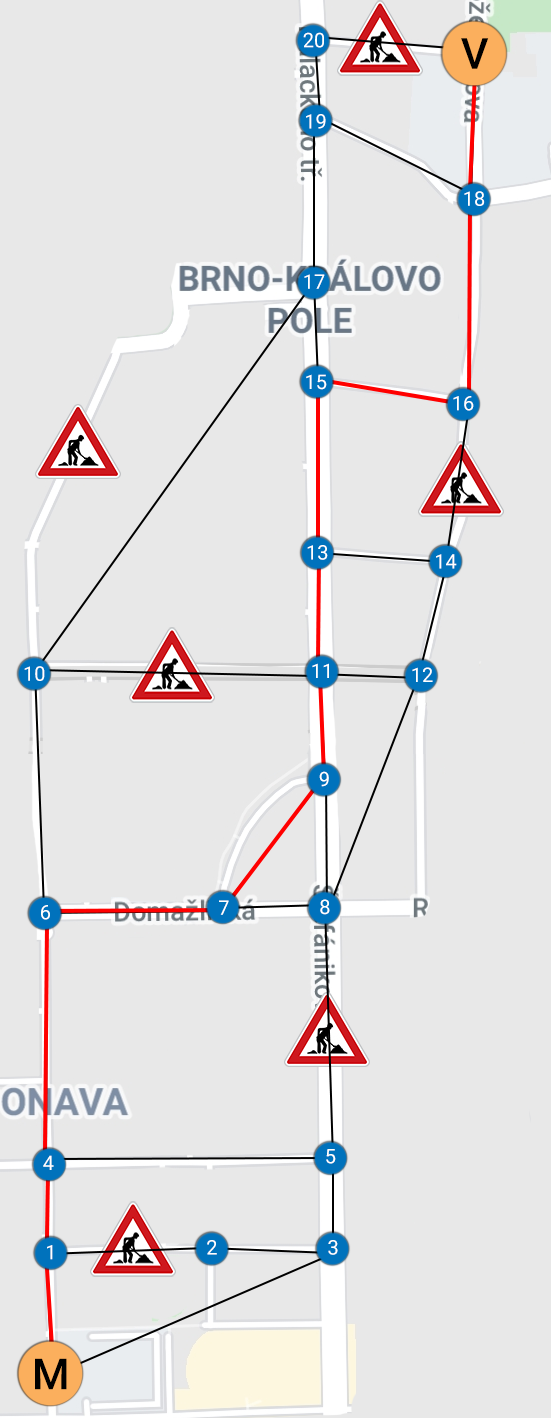
\includegraphics[height=0.9\textheight]{img/map/stud_res.png}
    }
\end{frame}

\begin{frame}\frametitle{Zdroje}
    \renewcommand\UrlFont{\ttfamily\footnotesize}
    
    \begin{itemize}
        \item Wikipedia: Dijkstra's algorithm\\
        \url{https://en.wikipedia.org/wiki/Dijkstra\%27s\_algorithm}
        \item L. Holík: Teorie grafů\\
        \url{http://www.fit.vutbr.cz/~lengal/idm/grafy-zaklady.pdf}
        \item L. Holík: Teorie grafů -- Grafové algoritmy\\
        \url{http://www.fit.vutbr.cz/~lengal/idm/grafy-algoritmy.pdf}
        \item Obrázky map vychází z~Google Map\\
        \url{http://maps.google.com/}
    \end{itemize}
\end{frame}

\bluepage{Děkuji za pozornost.}


\end{document}
